\documentclass[italian]{article}
%\usepackage{fontspec}
\usepackage{tikz}
\usetikzlibrary{positioning}
\usetikzlibrary{arrows,decorations.pathreplacing}
\begin{document}
    
    \section*{Significato dei dati trasmessi}
    
    Ogni quadrettino corrisponde ad un byte. Sono disponibili 16 bytes:
    
    \begin{itemize}
        \item 2 byte per descrivere il tipo di oggetto
        \item 2 byte per indicare l'ID dell'oggetto
        \item 8 byte per un valore numerico
        \item 4 bytes 'liberi' 
    \end{itemize}
    
    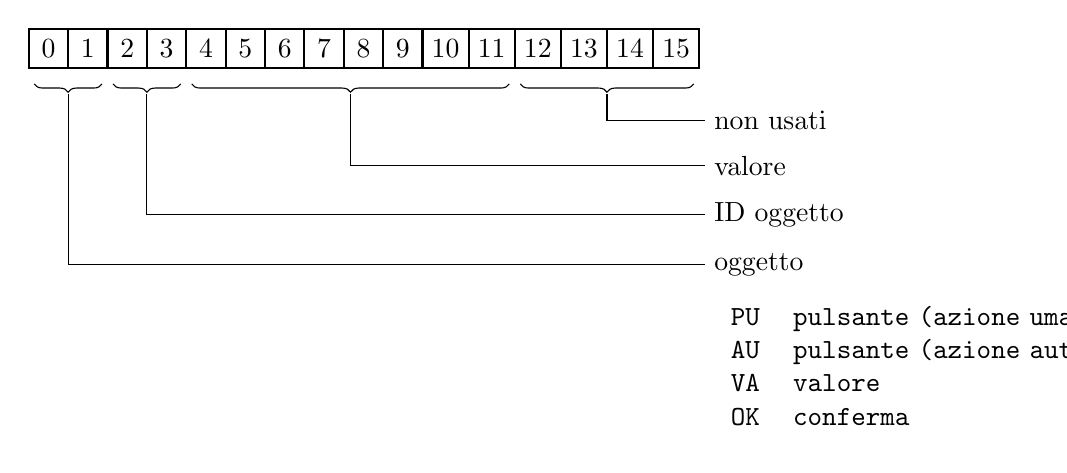
\begin{tikzpicture}[base/.style={draw,thick,minimum size=5mm,node distance=0pt,outer sep=0pt},altro/.style={text width=4cm,align=left,minimum size=0pt,node distance=3pt,outer sep=0pt}]
        \node[base](a){0};
        \node[base,right=of a,anchor=west](b){1};
        \node[base,right=of b,anchor=west](c){2};
        \node[base,right=of c,anchor=west](d){3};
        \node[base,right=of d,anchor=west](e){4};
        \node[base,right=of e,anchor=west](f){5};
        \node[base,right=of f,anchor=west](g){6};
        \node[base,right=of g,anchor=west](h){7};
        \node[base,right=of h,anchor=west](i){8};                        
        \node[base,right=of i,anchor=west](j){9};
        \node[base,right=of j,anchor=west](k){10};
        \node[base,right=of k,anchor=west](l){11};
        \node[base,right=of l,anchor=west](m){12}; 
        \node[base,right=of m,anchor=west](n){13};
        \node[base,right=of n,anchor=west](o){14};
        \node[base,right=of o,anchor=west](p){15};                
        %
        \coordinate[yshift=-2mm,xshift=2pt](aa) at (a.south west);
        \coordinate[yshift=-2mm,xshift=-2pt](bb) at (b.south east);
        %
        \coordinate[yshift=-2mm,xshift=2pt](cc) at (c.south west);
        \coordinate[yshift=-2mm,xshift=-2pt](dd) at (d.south east);
        %
        \coordinate[yshift=-2mm,xshift=2pt](ee) at (e.south west);
        \coordinate[yshift=-2mm,xshift=-2pt](ll) at (l.south east);
        %
        \coordinate[yshift=-2mm,xshift=2pt](mm) at (m.south west);
        \coordinate[yshift=-2mm,xshift=-2pt](pp) at (p.south east);        
        %
        \draw[decorate,decoration={brace,amplitude=3pt,mirror}] 
        (aa) --  node(x) {} (bb);
        \draw[decorate,decoration={brace,amplitude=3pt,mirror}] 
        (cc) --  node(y) {} (dd);
        \draw[decorate,decoration={brace,amplitude=3pt,mirror}] 
        (ee) --  node(z) {} (ll);
        \draw[decorate,decoration={brace,amplitude=3pt,mirror}] 
        (mm) --  node(w) {} (pp);
        %
        \node[altro,below right=of p,yshift=-10pt](sotto){non usati};
        \draw (w) |- (sotto);
        \node[altro,below =of sotto](sotto){valore};
        \draw (z) |- (sotto);
        \node[altro,below =of sotto](sotto){ID oggetto};
        \draw (y) |- (sotto);
        \node[altro,below =of sotto](sotto){oggetto};
        \draw (x) |- (sotto);  
        %
        \node[altro,below=of sotto]{\texttt{\begin{tabular}{ll}
            PU & pulsante (azione umana)\\
            AU & pulsante (azione automatica)\\            
            VA & valore\\
            OK & conferma\\
            \end{tabular}}};
    \end{tikzpicture}
    
    \textbf{Nota:} Un interruttore viene trasmesso come due pulsanti: uno per accendere l'altro per spegnere
    
    \section*{Esempi}
    
    Se viene trasmesso: \texttt{PU43000000000000} significa che è stato premuto il pulsante 43.
    
    L'unità in ascolto leggerà questo evento e prima di eseguire il suo compito  potrà mandare un segnale di conferma: \texttt{OK76000000000000}; significherà appunto che l'unità 76 (lo stesso circuito stampato manderà sempre questo stesso numero) ha ricevuto il comando.
    
    Il suo compito potrà essere:
    
    \begin{itemize}
        \item accendere/spegnere una luce (operazione solo sul pin)
        \item ritrasmettere (anche temporizzato autonomamente)\footnote{può essere che sia meglio di no: ogni volta conviene interrogare lo stato} il valore di un sensore, lo stato di un pin, lo stato interno di esecuzione di una azione (esempio pfSense).
    \end{itemize}
    
%    \section*{Dati trasmessi}
%    
%    \begin{itemize}
%        \item pulsante premuto = X
%        \item ricevuto
%        \item valore analogico vale Y [0/9999]
%        \item valore digitale vale [0/1]
%    \end{itemize}
%    
%    \begin{itemize}
%        \item identificazione del mittente (numero)
%        \item identificazione dell'oggetto (pulsante, ricevuto, valore)
%        \item valore trasmesso
%    \end{itemize}
%    
%    \section*{Studio}
%    
%\begin{itemize}
%        \item Un interruttore viene trasmesso come due pulsanti: uno per accendere l'altro per spegnere
%\end{itemize}
%    
%    \begin{itemize}
%        \item \texttt{PU\textbf{44}00000000} pulsante \textbf{44} premuto
%        \item \texttt{PU\textbf{01}00000000} pulsante \textbf{01} premuto
%        \item \texttt{PU\textbf{XX}00000000} pulsante \textbf{XX} premuto
%        \item \texttt{VA\textbf{23}0000\textbf{1234}} valore sensore \textbf{23} vale 1234
%        \item \texttt{OK\textbf{03}00000001} ok, unità \textbf{03} ha ricevuto comando
%    \end{itemize}
%        
%    \begin{tabular}{lcccccccccccc}
%        
%    \end{tabular}
\end{document}
